% Options for packages loaded elsewhere
\PassOptionsToPackage{unicode}{hyperref}
\PassOptionsToPackage{hyphens}{url}
%
\documentclass[
]{book}
\usepackage{lmodern}
\usepackage{amssymb,amsmath}
\usepackage{ifxetex,ifluatex}
\ifnum 0\ifxetex 1\fi\ifluatex 1\fi=0 % if pdftex
  \usepackage[T1]{fontenc}
  \usepackage[utf8]{inputenc}
  \usepackage{textcomp} % provide euro and other symbols
\else % if luatex or xetex
  \usepackage{unicode-math}
  \defaultfontfeatures{Scale=MatchLowercase}
  \defaultfontfeatures[\rmfamily]{Ligatures=TeX,Scale=1}
\fi
% Use upquote if available, for straight quotes in verbatim environments
\IfFileExists{upquote.sty}{\usepackage{upquote}}{}
\IfFileExists{microtype.sty}{% use microtype if available
  \usepackage[]{microtype}
  \UseMicrotypeSet[protrusion]{basicmath} % disable protrusion for tt fonts
}{}
\makeatletter
\@ifundefined{KOMAClassName}{% if non-KOMA class
  \IfFileExists{parskip.sty}{%
    \usepackage{parskip}
  }{% else
    \setlength{\parindent}{0pt}
    \setlength{\parskip}{6pt plus 2pt minus 1pt}}
}{% if KOMA class
  \KOMAoptions{parskip=half}}
\makeatother
\usepackage{xcolor}
\IfFileExists{xurl.sty}{\usepackage{xurl}}{} % add URL line breaks if available
\IfFileExists{bookmark.sty}{\usepackage{bookmark}}{\usepackage{hyperref}}
\hypersetup{
  pdftitle={Python for social and experimental psychology},
  pdfauthor={Alexander Pastukhov},
  hidelinks,
  pdfcreator={LaTeX via pandoc}}
\urlstyle{same} % disable monospaced font for URLs
\usepackage{color}
\usepackage{fancyvrb}
\newcommand{\VerbBar}{|}
\newcommand{\VERB}{\Verb[commandchars=\\\{\}]}
\DefineVerbatimEnvironment{Highlighting}{Verbatim}{commandchars=\\\{\}}
% Add ',fontsize=\small' for more characters per line
\usepackage{framed}
\definecolor{shadecolor}{RGB}{248,248,248}
\newenvironment{Shaded}{\begin{snugshade}}{\end{snugshade}}
\newcommand{\AlertTok}[1]{\textcolor[rgb]{0.94,0.16,0.16}{#1}}
\newcommand{\AnnotationTok}[1]{\textcolor[rgb]{0.56,0.35,0.01}{\textbf{\textit{#1}}}}
\newcommand{\AttributeTok}[1]{\textcolor[rgb]{0.77,0.63,0.00}{#1}}
\newcommand{\BaseNTok}[1]{\textcolor[rgb]{0.00,0.00,0.81}{#1}}
\newcommand{\BuiltInTok}[1]{#1}
\newcommand{\CharTok}[1]{\textcolor[rgb]{0.31,0.60,0.02}{#1}}
\newcommand{\CommentTok}[1]{\textcolor[rgb]{0.56,0.35,0.01}{\textit{#1}}}
\newcommand{\CommentVarTok}[1]{\textcolor[rgb]{0.56,0.35,0.01}{\textbf{\textit{#1}}}}
\newcommand{\ConstantTok}[1]{\textcolor[rgb]{0.00,0.00,0.00}{#1}}
\newcommand{\ControlFlowTok}[1]{\textcolor[rgb]{0.13,0.29,0.53}{\textbf{#1}}}
\newcommand{\DataTypeTok}[1]{\textcolor[rgb]{0.13,0.29,0.53}{#1}}
\newcommand{\DecValTok}[1]{\textcolor[rgb]{0.00,0.00,0.81}{#1}}
\newcommand{\DocumentationTok}[1]{\textcolor[rgb]{0.56,0.35,0.01}{\textbf{\textit{#1}}}}
\newcommand{\ErrorTok}[1]{\textcolor[rgb]{0.64,0.00,0.00}{\textbf{#1}}}
\newcommand{\ExtensionTok}[1]{#1}
\newcommand{\FloatTok}[1]{\textcolor[rgb]{0.00,0.00,0.81}{#1}}
\newcommand{\FunctionTok}[1]{\textcolor[rgb]{0.00,0.00,0.00}{#1}}
\newcommand{\ImportTok}[1]{#1}
\newcommand{\InformationTok}[1]{\textcolor[rgb]{0.56,0.35,0.01}{\textbf{\textit{#1}}}}
\newcommand{\KeywordTok}[1]{\textcolor[rgb]{0.13,0.29,0.53}{\textbf{#1}}}
\newcommand{\NormalTok}[1]{#1}
\newcommand{\OperatorTok}[1]{\textcolor[rgb]{0.81,0.36,0.00}{\textbf{#1}}}
\newcommand{\OtherTok}[1]{\textcolor[rgb]{0.56,0.35,0.01}{#1}}
\newcommand{\PreprocessorTok}[1]{\textcolor[rgb]{0.56,0.35,0.01}{\textit{#1}}}
\newcommand{\RegionMarkerTok}[1]{#1}
\newcommand{\SpecialCharTok}[1]{\textcolor[rgb]{0.00,0.00,0.00}{#1}}
\newcommand{\SpecialStringTok}[1]{\textcolor[rgb]{0.31,0.60,0.02}{#1}}
\newcommand{\StringTok}[1]{\textcolor[rgb]{0.31,0.60,0.02}{#1}}
\newcommand{\VariableTok}[1]{\textcolor[rgb]{0.00,0.00,0.00}{#1}}
\newcommand{\VerbatimStringTok}[1]{\textcolor[rgb]{0.31,0.60,0.02}{#1}}
\newcommand{\WarningTok}[1]{\textcolor[rgb]{0.56,0.35,0.01}{\textbf{\textit{#1}}}}
\usepackage{longtable,booktabs}
% Correct order of tables after \paragraph or \subparagraph
\usepackage{etoolbox}
\makeatletter
\patchcmd\longtable{\par}{\if@noskipsec\mbox{}\fi\par}{}{}
\makeatother
% Allow footnotes in longtable head/foot
\IfFileExists{footnotehyper.sty}{\usepackage{footnotehyper}}{\usepackage{footnote}}
\makesavenoteenv{longtable}
\usepackage{graphicx}
\makeatletter
\def\maxwidth{\ifdim\Gin@nat@width>\linewidth\linewidth\else\Gin@nat@width\fi}
\def\maxheight{\ifdim\Gin@nat@height>\textheight\textheight\else\Gin@nat@height\fi}
\makeatother
% Scale images if necessary, so that they will not overflow the page
% margins by default, and it is still possible to overwrite the defaults
% using explicit options in \includegraphics[width, height, ...]{}
\setkeys{Gin}{width=\maxwidth,height=\maxheight,keepaspectratio}
% Set default figure placement to htbp
\makeatletter
\def\fps@figure{htbp}
\makeatother
\setlength{\emergencystretch}{3em} % prevent overfull lines
\providecommand{\tightlist}{%
  \setlength{\itemsep}{0pt}\setlength{\parskip}{0pt}}
\setcounter{secnumdepth}{5}
\usepackage{booktabs}
\usepackage[]{natbib}
\bibliographystyle{apalike}

\title{Python for social and experimental psychology}
\author{Alexander Pastukhov}
\date{2020-10-27}

\begin{document}
\maketitle

{
\setcounter{tocdepth}{1}
\tableofcontents
}
\hypertarget{introduction}{%
\chapter*{Introduction}\label{introduction}}
\addcontentsline{toc}{chapter}{Introduction}

\hypertarget{about-the-seminar}{%
\section*{About the seminar}\label{about-the-seminar}}
\addcontentsline{toc}{section}{About the seminar}

This is a material for \emph{Python for social and experimental psychology} seminar. Each chapter covers a single seminar, introducing necessary ideas and is accompanied by a notebook with exercises, which you need to complete and submit. The material assumes no foreknowledge of Python or programming from the reader. Its purpose is to gradually build up your knowledge and allow you to create more and more complex games. Yes, games! Of course, the real research is about performing experiments but there is little difference between the two. The basic ingredients are the same and, arguably, experiments are just boring games. And, be assured, if you can program a game, you certainly can program an experiment.

We will start with simple \emph{Guess a Number} text-only game with first you and then the computer doing the guessing. Next, we will implement a classic \emph{Hunt the Wumpus} text adventure game that will require use of more complex structures. Once we master the basics, we will up the ante by making a video game with graphics and sounds using \href{https://psychopy.org/}{PsychoPy} library to code a classic \emph{Memory Game}. Finally, we will create a more dynamic game by making a clone of a \emph{Flappy Bird}.

Remember that throughout the seminar you can and should(!) always ask me whenever something is unclear, you do not understand a concept or logic behind certain code. Do not hesitate to write me in the team or (better) directly to me in the chat (in the latter case, the notifications are harder miss and we don't spam others with our conversation).

You will need to submit your assignment one day before the next seminar (Tuesday before noon at the latest), so I would have time evaluate it and provide feedback.

As a final assignment, you will need to program a (currently mysterious) video game, which will only require the material covered by the seminar. Please inform me, If you require a grade, as then I will create a more specific description for you to have a clear understanding of how the program will be graded.

\hypertarget{note-on-exercises}{%
\section*{Note on exercises}\label{note-on-exercises}}
\addcontentsline{toc}{section}{Note on exercises}

In many exercises your will be not writing the code but understanding it. Your job in this case is ``to think like a computer''. Your advantage is that computers are very dumb, so instructions for them must be written in very simple, clear, and unambiguous way. This means that, with practice, reading code is easy for a human (well, reading a well-written code is easy, you will eventually encounter ``spagetti-code'' which is easier to rewrite from scratch than to understand). In each case, you simply go line-by-line, doing all computations by hand and writing down values stored in the variables (if there are too many to keep track of). Once you go through code in this manner, it will be completely transparent for you. No mysteries should remain, you should have no doubts or uncertainty about any(!) line. Moreover, then you can run the code and check that the values you are getting from computer match yours. Any difference means you made a mistake and code is working differently from how you think it does. In any case, \textbf{if you not 100\% sure about any line of code, ask me, so we can go through it together!}

In a sense, this is the most important programming skill. It is impossible to learn how to write, if you cannot read first! Moreover, when programming you will probably spend more time reading the code and making sure that it works correctly than writing the new code. Thus, use this opportunity to practice and never use the code that you do not understand completely. So do use \href{https://stackoverflow.com/}{stackoverflow} but do make sure you understand the code you copied!

\hypertarget{why-python}{%
\section*{Why Python?}\label{why-python}}
\addcontentsline{toc}{section}{Why Python?}

The ultimate goal of this seminar is to teach you how to create an experiment for psychology research. There are many ways to achieve this end. You can use drag-and-drop systems either commercial like \href{https://www.neurobs.com/}{Presentation}, \href{https://www.sr-research.com/experiment-builder/}{Experiment Builder} or free like \href{https://psychopy.org/builder}{PsychoPy Bulder interface}. They have a much shallower learning curve, so you can start creating and running your experiments faster. However, the simplicity of their use has the price: They are fairly limited in which stimuli you can use and how you can control the presentation schedule, feedback, etc. Typically, they allow you to extend them by programming the desired behavior but you do need to know how to program to do this. Thus, I think that while these systems, in particular \href{https://psychopy.org/}{PsychoPy}, are great tools to quickly bang a simple experiment together, they are most useful if you understand how they create the code and how you would program it yourself. Then, you will not fill being limited by the software, as you know you can program something the default drag-and-drop won't allow, but you can always opt in, if drag-and-drop is sufficient but faster. At the end, it is about having options and creative freedom to program an experiment that will answer your research question, not an experiment that your software allows you to program.

We will learn programming in Python, which is a great language that combines simple and clear syntax with power and ability to tackle almost any problem. The advantage of learning Python, as compared to say Matlab, which is commonly used in neuroscience, is that it allows you do almost anything. In this seminar, we will concentrate on desktop experiments but you can use it for online experiments (\href{https://otree.readthedocs.io/en/latest/}{oTree}), scientific programming (\href{https://numpy.org/}{NumPy} and \href{https://www.scipy.org/}{SciPy}), data analysis (\href{https://pandas.pydata.org/}{pandas}), machine learning (\href{https://keras.io/}{keras}), website programming (\href{https://www.djangoproject.com/}{django}), computer vision (\href{https://opencv.org/}{OpenCV}), etc. Thus, learning Python will give you one of the most versitile programming tools that you can use for all stages of your research or work. And, Python is free, so you do not need to worry whether you or your future employer will be able to afford the license fees (a very real problem, if you use Matlab).

\hypertarget{getting-started}{%
\chapter*{Getting Started}\label{getting-started}}
\addcontentsline{toc}{chapter}{Getting Started}

\hypertarget{install-anaconda}{%
\section*{Installing Anaconda environment}\label{install-anaconda}}
\addcontentsline{toc}{section}{Installing Anaconda environment}

First, install \href{https://www.anaconda.com}{Anaconda}, a Python distribution that includes many packages and tools out-of-the-box, makes it easy to install new packages and keep them updated. Follow this \href{https://www.anaconda.com/products/individual}{link} and download the installer suitable for your platform. You can pick either 32- or 64-bit version but I would recommend the latter, so that we all have maximally similar setup (it won't really make a difference in practice, though). Follow the installer instructions and use defaults, unless you have reasons to modify them (e.g.~folder location, as the drive for the default choice may have limited available space, as in my case).

After installation you will have a new \emph{Anaconda3 (64-bit)} folder that contains links to programs.

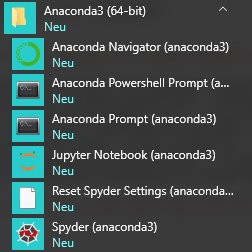
\includegraphics[width=3.5in]{images/anaconda-shortcuts}

You can use \emph{Anaconda Navigator} that allows you to choose a specific programming environment, including \href{https://jupyter.org/}{Jupyter Notebook} that we will use (not JupyterLab, it more versatile but we want to keep things simple at the beginning!). Alternatively, you can start \emph{Jupyter Notebook} directly from the start menu. Please read the \href{https://jupyter-notebook.readthedocs.io/en/stable/examples/Notebook/examples_index.html}{online documentation} to familiarize yourself with Jupyter Notebook basic interface, e.g.~how to create a new cell, run it, etc.

\hypertarget{install-vs-code}{%
\section*{Installing Visual Studio Code}\label{install-vs-code}}
\addcontentsline{toc}{section}{Installing Visual Studio Code}

\href{https://code.visualstudio.com/}{Visual Studio Code} is a lightweight free open-source editor with strong support for Python. We will start use it in earnest, once our programs grow to be sufficiently long and complex. At the early stages, we will mostly use Jupyter notebooks and I would recommend using Jupyter notebooks using the default browser-based editor you installed as part of \protect\hyperlink{install-anaconda}{Anaconda}. However, you can also work with Jupyter notebooks in VS Code \href{https://code.visualstudio.com/docs/python/jupyter-support}{directly}.

As in case of \protect\hyperlink{install-anaconda}{Anaconda}, download the installer for your platform and follow the instructions. Start VS Code and open any Python file, for example \href{other/empty.py}{this one} (use \texttt{Alt+click} to download it, ignore warnings, it is has only comments, so cannot harm you). When you open Python file for the first time, VS Code will suggest to install a Python extension. Do just that andinstall a linter as well when VS Code suggests that (\href{https://code.visualstudio.com/docs/python/linting}{linting} highlights syntactical and stylistic problems in your code, making it easier to write consistent clear code).

Once the Python extension is activated, you will see which Python interpreter is used (you can have more than one or you may use have multiple \href{https://docs.python.org/3/tutorial/venv.html}{virtual environments}).


\includegraphics[width=6.96in]{images/vscode-python-interpreter}
If the selected environment is the wrong one or you are simply not sure, click on it and it will open a drop-down list with all interpreters and environments you have. Consult VS Code \href{https://code.visualstudio.com/docs/python/environments}{online documentation} on environments, if you need to change/add/delete environment (the exact settings may change, so looking at constantly updated online documentation is wiser than copying it here, so it would be outdated quite soon).

\hypertarget{install-psychopy}{%
\section*{Installing PsychoPy}\label{install-psychopy}}
\addcontentsline{toc}{section}{Installing PsychoPy}

This step can wait until the first \protect\hyperlink{memory-game-01}{Memory Game} seminar.

Download and install \href{https://www.psychopy.org/download.html}{Standalone PsychoPy} version. You can install PsychoPy as a conda package or via pip but using it as a standalone would ensure that you have all necessary additional libraries and a builder interface for the future use. We will use PsychoPy's python environment in \protect\hyperlink{install-vs-code}{VS Code}.

\hypertarget{seminar01}{%
\chapter{Python basics}\label{seminar01}}

Before we start, create a folder called \emph{python-for-experiments} (or with some other more suitable but meaningful name) in you user folder (this is where Anaconda's Jupyter Notebook expect to find them). Download the \href{notebooks/Seminar\%2001.\%20Guess\%20the\%20number.ipynb}{exercise notebook} and put it in this folder. Open Jupyter Notebook (see \protect\hyperlink{getting-started}{Getting Started}, if you forgot how you do that), navigate to the folder you created and open the downloaded notebook. You will need to switch between explanations here and the exercises in the notebook, so keep them both open. The seminar contains the material introducing the concepts and tools that you require to implement the game step-by-step.

\hypertarget{variables}{%
\section{Variables}\label{variables}}

The first fundamental concept that we need to be acquainted with is \textbf{variable}. Variables are used to store information and you can think of it as a box with a name tag in which you can put something. The name tag on that the box is the name of the variable and its value what you store in it. For example, we can create a variable that stores the number of legs a game character has and we begin with a number typical for a human being.

\textbf{FIGURE!}

In Python, you would write

\begin{Shaded}
\begin{Highlighting}[]
\NormalTok{number\_of\_legs }\OperatorTok{=} \DecValTok{2}
\end{Highlighting}
\end{Shaded}

The \textbf{assignment statement} above has very simple structure \texttt{\textless{}variable-name\textgreater{}\ =\ \textless{}value\textgreater{}}. Variable name (name tag on the box) should be meaningful, it can start with letters or \_ and can contain letters, numbers, and \_ symbols but must have no spaces in them. Preferably, you should use \textbf{snake\_case} (all lower-case, underscore for spaces) to format your variable names. The \texttt{\textless{}value\textgreater{}} on the right side is a more complex story, as it can be simply hard-coded (as in example above), computed using other variables or the same variable, returned by a function, etc.

Using variables means that you can concentrate what corresponding values \textbf{mean} rather than worrying about what these values are. For example, the next time you need to compute something based on number of character's legs (e.g.~how many pairs of shoes does a character need), you can compute it based on current value of \texttt{number\_of\_legs} variable rather than assume that it is \texttt{1}.

\begin{Shaded}
\begin{Highlighting}[]
\CommentTok{\# BAD: why 1? Is it because the character has two legs or}
\CommentTok{\# because we issue one pair of shoes per character irrespective of}
\CommentTok{\# their actual number of legs?}
\NormalTok{pairs\_of\_shoes }\OperatorTok{=} \DecValTok{1}

\CommentTok{\# BETTER!}
\NormalTok{pairs\_of\_shoes }\OperatorTok{=}\NormalTok{ number\_of\_legs }\OperatorTok{/} \DecValTok{2}
\end{Highlighting}
\end{Shaded}

Variables also gives you flexibility. Their values can change during the program run: player's score is increasing, number of lives decreasing, number of spells it can cast grows or falls depending on their use, etc. Yet, you can use the value in the variable to perform necessary computations. For example, here is a slightly extended \texttt{number\_of\_shoes} example.

\begin{Shaded}
\begin{Highlighting}[]
\NormalTok{number\_of\_legs }\OperatorTok{=} \DecValTok{2}

\CommentTok{\# ...}
\CommentTok{\# something happens and our character is turned into an octopus}
\NormalTok{number\_of\_legs }\OperatorTok{=} \DecValTok{8}
\CommentTok{\# ...}

\CommentTok{\# the same code still works and we know the correct number of pairs of shoes}
\NormalTok{pairs\_of\_shoes }\OperatorTok{=}\NormalTok{ number\_of\_legs }\OperatorTok{/} \DecValTok{2}
\end{Highlighting}
\end{Shaded}

As noted above, you can think about a variable as box labeled box you can store something in. That means that you can always ``throw away'' the old value and put something new. In case of variables, the ``throwing away'' part happens automatically, as the new value overwrites the old one. Check yourself, what will be final value of the variable in the code below? Go to exercise \#1 in the notebook.

\begin{Shaded}
\begin{Highlighting}[]
\NormalTok{number\_of\_legs }\OperatorTok{=} \DecValTok{2}
\NormalTok{number\_of\_legs }\OperatorTok{=} \DecValTok{5}
\NormalTok{number\_of\_legs }\OperatorTok{=} \DecValTok{1}
\NormalTok{number\_of\_legs}
\end{Highlighting}
\end{Shaded}

As you have already seen, you can \emph{compute} a value instead of specifying it. What would be the answer here? Do exercise \#2 in the notebook.

\begin{Shaded}
\begin{Highlighting}[]
\NormalTok{number\_of\_legs }\OperatorTok{=} \DecValTok{2} \OperatorTok{*} \DecValTok{2}
\NormalTok{number\_of\_legs }\OperatorTok{=} \DecValTok{7} \OperatorTok{{-}} \DecValTok{2}
\NormalTok{number\_of\_legs}
\end{Highlighting}
\end{Shaded}

A \textbf{very important} rule that you must keep in mind when understanding assignments: the right side expression is evaluated first until the final value is computed, only when the computation finished the value is assigned to the variable (put in the box). What this means is that you can use the same variable on \textbf{both} sides! Let's take a look at this code:

\begin{Shaded}
\begin{Highlighting}[]
\NormalTok{x }\OperatorTok{=} \DecValTok{2}
\NormalTok{y }\OperatorTok{=} \DecValTok{5}
\NormalTok{x }\OperatorTok{=}\NormalTok{ x }\OperatorTok{+}\NormalTok{ y }\OperatorTok{{-}} \DecValTok{4}
\end{Highlighting}
\end{Shaded}

What happens when computer evaluates the following line?

\begin{Shaded}
\begin{Highlighting}[]
\NormalTok{x }\OperatorTok{=}\NormalTok{ x }\OperatorTok{+}\NormalTok{ y }\OperatorTok{{-}} \DecValTok{4}
\end{Highlighting}
\end{Shaded}

First, it takes \emph{current} values of all variables (\texttt{x} and \texttt{y}) and substitutes them into the expression. After that internal step, the expression looks like

\begin{Shaded}
\begin{Highlighting}[]
\NormalTok{x }\OperatorTok{=} \DecValTok{2} \OperatorTok{+} \DecValTok{5} \OperatorTok{{-}} \DecValTok{4}
\end{Highlighting}
\end{Shaded}

Then, it computes the arithmetic expression for the right side and stores that new value in \texttt{x}

\begin{Shaded}
\begin{Highlighting}[]
\NormalTok{x }\OperatorTok{=} \DecValTok{3}
\end{Highlighting}
\end{Shaded}

Switch to the notebook and do exercise \#3 to make sure you understand this.

\hypertarget{constants}{%
\section{Constants}\label{constants}}

Although the real power of variables is that you can change their value, you should use them even if the value remains constant. There are no constants in Python, rather the agreement is that their names should be all \texttt{UPPER\_CASE}. So, if number of legs stays constant throughout the game, you should highlight that constancy and write

\begin{Shaded}
\begin{Highlighting}[]
\NormalTok{NUMBER\_OF\_LEGS }\OperatorTok{=} \DecValTok{2}
\end{Highlighting}
\end{Shaded}

I strongly recommend using constants and avoid hardcoding the values. First, if you have several identical values that mean different things (2 legs, 2 eyes, 2 ears, 2 vehicles per character, etc.), seeing a \texttt{2} in the code won't tell you what does this \texttt{2} mean (the legs? the ears? the score multiplier?). You can, of course, figure it out based on the code that uses this number but you could spare yourself that extra effort and use a constant instead. Then, you just read its name and the meaning of the value becomes apparent. Second, if you decide to \emph{change} that value (say, our main character is now a tripod), when using a constant means you have only one place to worry about, the rest of the code stays as is. If you hard-coded that number, you are in for an exciting (not really) and long search-and-replace throughout the entire code.

\hypertarget{value-types}{%
\section{Value types}\label{value-types}}

So far, we only used integer numeric values (1, 2, 5, 1000\ldots). Although, Python supports \href{https://docs.python.org/3/library/stdtypes.html}{many different value types} but we will concentrate on a small subset of them first:

\begin{itemize}
\tightlist
\item
  integer numbers, we already used, e.g.~\texttt{-1}, \texttt{100000}, \texttt{42}.
\item
  float numbers that can take any real value, e.g.~\texttt{42.0}, \texttt{3.14159265359}, \texttt{2.71828}.
\item
  strings that can store text. The text is enclosed between either paired quotes \texttt{"some\ text"} or apostrophes \texttt{\textquotesingle{}some\ text\textquotesingle{}}. This means that you can use quotes or apostrophes inside the string, as long as its is enclosed by the alternative. E.g., \texttt{"students\textquotesingle{}\ homework"} (enclosed in \texttt{"}, apostrophe \texttt{\textquotesingle{}} inside) or \texttt{\textquotesingle{}"All\ generalizations\ are\ false,\ including\ this\ one."\ Mark\ Twain\textquotesingle{}} (quotation enclosed by apostrophes).
\item
  logical / Boolean values that are either \texttt{True} or \texttt{False}.
\end{itemize}

When using a variable it is important that you know what type of value it stores. In some cases, Python will automatically convert values between certain types, e.g.~any integer value is also a real value, so conversion from \texttt{1} to \texttt{1.0} is mostly trivial and automatic. However, in other cases you may need to use explicit conversion. Go to exercise \#4 and think about which code will run and which will throw an error due to incompatible types?

\begin{Shaded}
\begin{Highlighting}[]
\DecValTok{5} \OperatorTok{+} \FloatTok{2.0}
\CommentTok{\textquotesingle{}5\textquotesingle{}} \OperatorTok{+} \DecValTok{2}
\CommentTok{\textquotesingle{}5\textquotesingle{}} \OperatorTok{+} \StringTok{\textquotesingle{}2\textquotesingle{}}
\CommentTok{\textquotesingle{}5\textquotesingle{}} \OperatorTok{+} \VariableTok{True}
\DecValTok{5} \OperatorTok{+} \VariableTok{True}
\end{Highlighting}
\end{Shaded}

Surprised by the last one? This is because internally, \texttt{True} is also \texttt{1} and \texttt{False} is \texttt{0}!

You can explicitly convert from one type to another using special functions (we will explore these functions in greater detail below). For example, to turn a number or a logical value into a string, you simply write \texttt{str(\textless{}value\textgreater{})}. In examples below, what would be the result (go to exercise \#5 in the notebook)?

\begin{Shaded}
\begin{Highlighting}[]
\BuiltInTok{str}\NormalTok{(}\DecValTok{10} \OperatorTok{/} \DecValTok{2}\NormalTok{)}
\BuiltInTok{str}\NormalTok{(}\FloatTok{2.5} \OperatorTok{+} \VariableTok{True}\NormalTok{)}
\BuiltInTok{str}\NormalTok{(}\VariableTok{True}\NormalTok{)}
\end{Highlighting}
\end{Shaded}

Similarly, you can convert to a logical/Boolean variable using \texttt{bool(\textless{}value\textgreater{})} function. The rules are simple, for numeric values \texttt{0} is \texttt{False}, any other non-zero value is converted to \texttt{True}. For string, an empty string \texttt{\textquotesingle{}\textquotesingle{}} is evaluated to \texttt{False} and non-empty string is converted to \texttt{True}. What would be the output in the examples below (go to exercise \#6 in the notebook)?

\begin{Shaded}
\begin{Highlighting}[]
\BuiltInTok{bool}\NormalTok{(}\OperatorTok{{-}}\DecValTok{10}\NormalTok{)}
\BuiltInTok{bool}\NormalTok{(}\FloatTok{0.0}\NormalTok{)}

\NormalTok{secret\_message }\OperatorTok{=} \StringTok{\textquotesingle{}\textquotesingle{}}
\BuiltInTok{bool}\NormalTok{(secret\_message)}

\BuiltInTok{bool}\NormalTok{(}\StringTok{\textquotesingle{}False\textquotesingle{}}\NormalTok{)}
\end{Highlighting}
\end{Shaded}

Converting to integer or float numbers is trickier. The simplest case is from logical to integer/float, as \texttt{True} gives you \texttt{int(True)} is \texttt{1} and \texttt{float(True)} is \texttt{1.0} and \texttt{False} gives you \texttt{0}/\texttt{0.0}. When converting from float to integer, Python simply drops the fractional part (not rounding!). When converting a string, it must be a valid number of the corresponding type or the error is thrown. E.g., you can convert a string like \texttt{"123"} to and integer or a float but this won't work for \texttt{"a123"}. Moreover, you can convert \texttt{"123.4"} to floating-point number but not to an integer, as it has fractional part in it. Given all this, which cells would work and what output would they give (go to exercise \#7 in the notebook)?

\begin{Shaded}
\begin{Highlighting}[]
\BuiltInTok{float}\NormalTok{(}\VariableTok{False}\NormalTok{)}
\BuiltInTok{int}\NormalTok{(}\OperatorTok{{-}}\FloatTok{3.3}\NormalTok{)}
\BuiltInTok{float}\NormalTok{(}\StringTok{"67.8"}\NormalTok{)}
\BuiltInTok{int}\NormalTok{(}\StringTok{"123+3"}\NormalTok{)}
\end{Highlighting}
\end{Shaded}

\hypertarget{printing-output}{%
\section{Printing output}\label{printing-output}}

To print the value, you need you use \texttt{print()} function (we will talk about functions in greater detail later). In simplest case, you pass the value and it will be printed out.

\begin{Shaded}
\begin{Highlighting}[]
\BuiltInTok{print}\NormalTok{(}\DecValTok{5}\NormalTok{)}
\end{Highlighting}
\end{Shaded}

\begin{verbatim}
## 5
\end{verbatim}

or

\begin{Shaded}
\begin{Highlighting}[]
\BuiltInTok{print}\NormalTok{(}\StringTok{"five"}\NormalTok{)}
\end{Highlighting}
\end{Shaded}

\begin{verbatim}
## five
\end{verbatim}

Of course, you already know about the variables, so rather that putting the value directly, you can pass a variable instead and it is its value that will be printed out.

\begin{Shaded}
\begin{Highlighting}[]
\NormalTok{number\_of\_pancakes }\OperatorTok{=} \DecValTok{10}
\BuiltInTok{print}\NormalTok{(number\_of\_pancakes)}
\end{Highlighting}
\end{Shaded}

\begin{verbatim}
## 10
\end{verbatim}

or

\begin{Shaded}
\begin{Highlighting}[]
\NormalTok{breakfast }\OperatorTok{=} \StringTok{"pancakes"}
\BuiltInTok{print}\NormalTok{(breakfast)}
\end{Highlighting}
\end{Shaded}

\begin{verbatim}
## pancakes
\end{verbatim}

You can also pass more than one value/variable to the print function and all the values will be printed one after another. For example, if we want to tell the user what did I had for breakfast and just how many of those, we can do

\begin{Shaded}
\begin{Highlighting}[]
\NormalTok{breakfast }\OperatorTok{=} \StringTok{"pancakes"}
\NormalTok{number\_of\_items }\OperatorTok{=} \DecValTok{10}
\BuiltInTok{print}\NormalTok{(breakfast, number\_of\_items)}
\end{Highlighting}
\end{Shaded}

\begin{verbatim}
## pancakes 10
\end{verbatim}

Go to exercise \#8 and figure out what will be printed by the code below:

\begin{Shaded}
\begin{Highlighting}[]
\NormalTok{dinner }\OperatorTok{=} \StringTok{"stake"}
\NormalTok{count }\OperatorTok{=} \DecValTok{4}
\NormalTok{desert }\OperatorTok{=} \StringTok{"cupcakes"}

\BuiltInTok{print}\NormalTok{(count, dinner, count, desert)}
\end{Highlighting}
\end{Shaded}

However, you probably would want to be more explicit, when you print out the information. For example, imagine you have these three variables:

\begin{Shaded}
\begin{Highlighting}[]
\NormalTok{meal }\OperatorTok{=} \StringTok{"breakfast"}
\NormalTok{dish }\OperatorTok{=} \StringTok{"pancakes"}
\NormalTok{count }\OperatorTok{=} \DecValTok{10}
\end{Highlighting}
\end{Shaded}

You could, of course do \texttt{print(meal,\ dish,\ count)} but it would be nicer to print

``\emph{I had \textbf{10 pancakes} for \textbf{breakfast}}''

there items in bold would be the inserted variables' values. For this, we need to use string formatting. Please note that the string formatting is not specific to printing, you can create a new string value via formatting and store it in a variable (without printing it out) or print it out (without storing it).

\hypertarget{string-formatting}{%
\section{String formatting}\label{string-formatting}}

A great resource on string formatting in Python is \href{https://pyformat.info/}{pyformat.info}. As Python constantly evolves, it now has more than one way to format strings. Below, I will introduce the ``old'' format that is based on classic string formatting used in \texttt{sprintf} function is C, Matlab, R, and many other programming languages. It is somewhat less flexible than a newer ones but for simple tasks the difference is negligible. Knowing the old format is useful because of its generality. If you want to learn alternatives, read at the link above.

The general call is \texttt{"a\ string\ with\ formatting"\%(tuple\ of\ values\ to\ be\ used\ during\ formatting)}.

In \texttt{"a\ string\ with\ formatting"}, you specify where you want to put the value via \texttt{\%} symbol that is followed by an \emph{optional} formatting info and the \emph{required} symbol that defines the \textbf{type} of the value. The type symbols are
* \texttt{s} for string
* \texttt{d} for an integer
* \texttt{f} for a float value, so that it is fully printed
* \texttt{g} for an optimally printed float value, so that scientific notation is used for large values (\emph{e.g.}, \texttt{10e5} instead of \texttt{100000}).

Here is an example of formatting a string using an integer:

\begin{Shaded}
\begin{Highlighting}[]
\BuiltInTok{print}\NormalTok{(}\StringTok{"I had }\SpecialCharTok{\%d}\StringTok{ pancakes for breakfast"}\OperatorTok{\%}\NormalTok{(}\DecValTok{10}\NormalTok{))}
\end{Highlighting}
\end{Shaded}

\begin{verbatim}
## I had 10 pancakes for breakfast
\end{verbatim}

You are not limited to a single value that you can put into a string. You can specify more locations via \texttt{\%} but you must make sure that you pass the right number of values. Before running it, can you figure out which call will actually work (and what will be the output ) and which will produce an error (go to exercise \#9)?

\begin{Shaded}
\begin{Highlighting}[]
\BuiltInTok{print}\NormalTok{(}\StringTok{\textquotesingle{}I had }\SpecialCharTok{\%d}\StringTok{ pancakes and either }\SpecialCharTok{\%d}\StringTok{  or }\SpecialCharTok{\%d}\StringTok{ stakes for dinner\textquotesingle{}}\OperatorTok{\%}\NormalTok{(}\DecValTok{2}\NormalTok{))}
\BuiltInTok{print}\NormalTok{(}\StringTok{\textquotesingle{}I had }\SpecialCharTok{\%d}\StringTok{ pancakes and }\SpecialCharTok{\%d}\StringTok{ stakes for dinner\textquotesingle{}}\OperatorTok{\%}\NormalTok{(}\DecValTok{7}\NormalTok{, }\DecValTok{10}\NormalTok{))}
\BuiltInTok{print}\NormalTok{(}\StringTok{\textquotesingle{}I had }\SpecialCharTok{\%d}\StringTok{ pancakes and }\SpecialCharTok{\%d}\StringTok{ stakes for dinner\textquotesingle{}}\OperatorTok{\%}\NormalTok{(}\DecValTok{1}\NormalTok{, }\DecValTok{7}\NormalTok{, }\DecValTok{10}\NormalTok{))}
\end{Highlighting}
\end{Shaded}

In case of real values you have two options: \texttt{\%f} and \texttt{\%g}. The latter uses scientific notation (e.g.~\texttt{1e10} for \texttt{10000000000}) to make the representation more compact. To get a better feeling for the difference do exercise \#10.

These is much more to formatting and you can read about it at \href{https://pyformat.info/}{pyformat.info}. However, these basics are sufficient for us to start programming our first game during the next seminar. Don't forget to submit your exercise notebook and see you next time!

\hypertarget{seminar02}{%
\chapter{Guess the Number}\label{seminar02}}

\hypertarget{game-description}{%
\section{Game description}\label{game-description}}

We will program a game where one participant (computer) picks the number within a certain range, say, between 1 and 10 and the other participant (player) is trying to guess it. After every guess, the first participant (computer) responds whether the actual number is lower than a guess, higher than a guess, or matches it. The game is over when the player correctly guess the number or (in the later version of the game) runs out of attempts.

\end{document}
